\chapter{Standar Perlengkapan}

Dalam pertempuran untuk membuat jurnal ilmiah maka diharapkan memeiliki alat bantu berupa aplikasi. Alat bantu aplikasi tersebut berguna untuk proses mempercepat penulisan jurnal ilmiah. Selain aplikasi juga harus memiliki beberapa akun yang berfungsi untuk memperluas jaringan kolaborasi publikasi ilmiah. Beberapa alat bantu aplikasi dan akun yang wajib dimiliki antara lain :
\begin{enumerate}
\item Grammarly dengan akun premium.
\item akun sharelatex dan latex compiler di komputer.
\item akun researchgate
\item Profile Google Scholar
\item Profile orcid.org
\item Aplikasi dan akun mendeley
\end{enumerate}
Kemudian yang tidak kalah penting adalah memiliki mentor yang mempunya H-Index diatas 10. Memiliki mentor berfungsi untuk mempercepat proses pematangan diri agar siap produktif membuat jurnal. Lebih bagus lagi mentor dari luar negeri. Diharapkan memiliki minimal 3 mentor dari lintas institusi pendidikan.

\section{Pencarian Topik}
Satu-satunya cara adalah untuk mendapatkan topik publikasi adalah dengan membaca jurnal 5 tahun terakhir terindex scopus minimal sebanyak 15 buah. Carilah jurnal dengan pencarian  kata kunci sesuai dengan topik yang kita inginkan. Kemudian tuangkan dalam slide presentasi dengan satu halaman setiap jurnal terdiri dari judul, masalah, metode, hasil.

\section{Pengambilan BibTex}
Untuk mendapatkan BibTex yang nantinya akan di taruh di Latex Kita. Maka kita bisa menggunakan Google Scholar. Google Scholar memiliki alamat scholar.google.com kemudian kita akan dihantarkan pada halaman pencarian seperti terlihat pada gambar \ref{gsutama}. Dari sini kita cari terlebih dahulu judul dari artikel yang sudah kita baca di kotak pencarian(gambar \ref{caritopik}). Setelah itu kita klik tanda kutip seperti gambar \ref{pilihtandakutip}. Terbuka area putih di depannya dan pilih menu bibtex di gambar \ref{hasiltandakutip}. Dan selanjutkan tinggal menyalin dari keluaran bibtex scholar yang tampak seperti gambar \ref{hasilbibtex} ke file references.bib. Dan setelah itu kita bisa memanggil untuk mensitasi di file latex kita dengan tag \verb|\cite{oja1983descriptive}|.

\begin{figure}[ht]
        \centerline{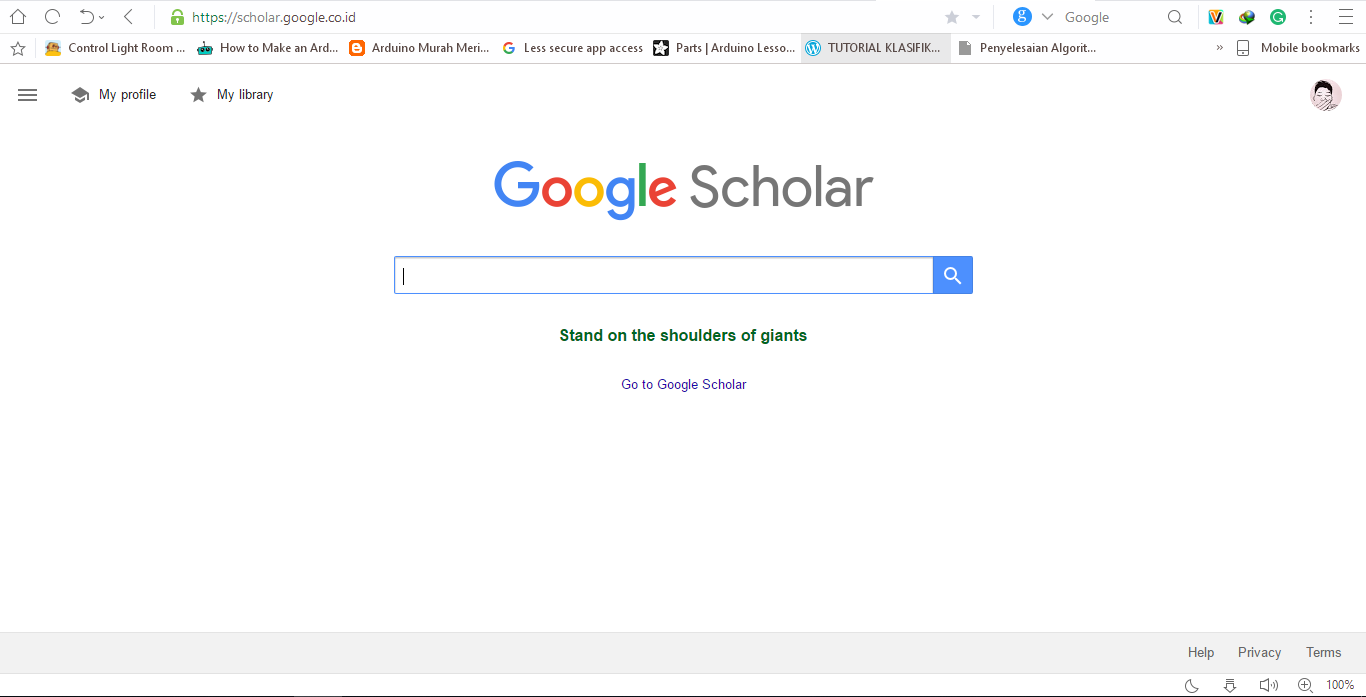
\includegraphics[width=1\textwidth]{figures/lamanscholar}}
        \caption{Laman Google Scholar}
		\label{gsutama}
\end{figure}

\begin{figure}[ht]
       \centerline{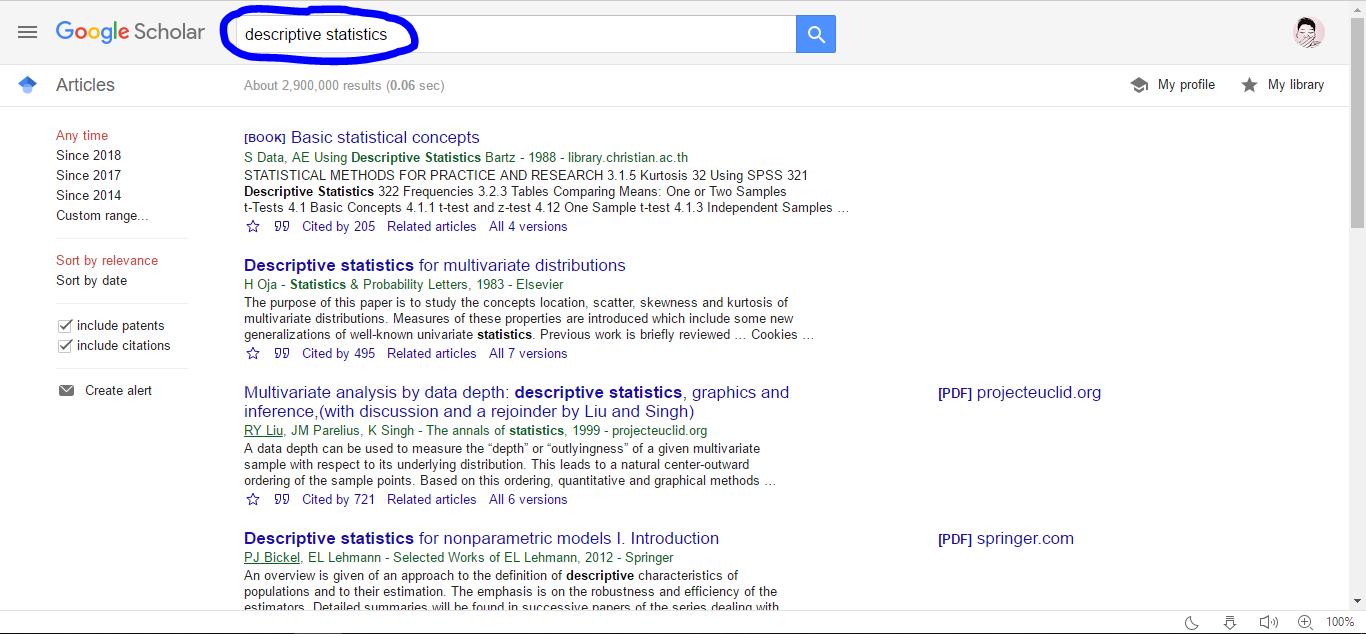
\includegraphics[width=1\textwidth]{figures/pencarianscholar}}
       \caption{Hasil Pencarian Topik}
		\label{caritopik}
\end{figure}

\begin{figure}[ht]
        \centerline{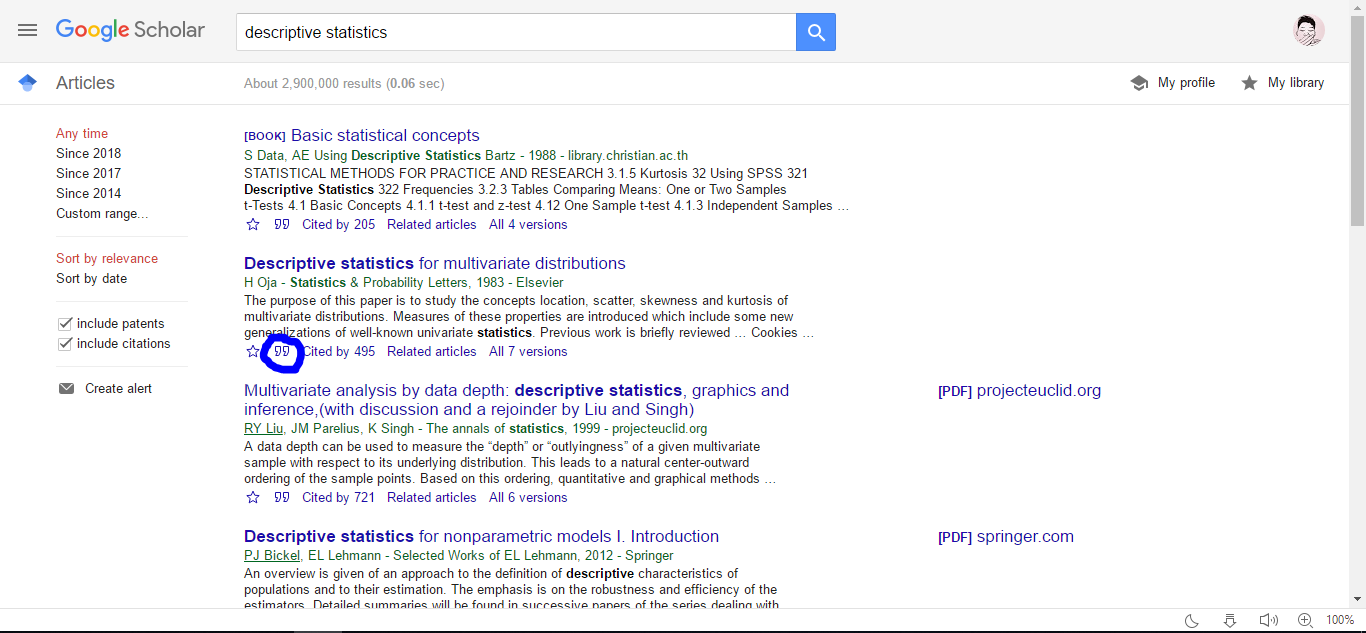
\includegraphics[width=1\textwidth]{figures/pilihtandakutip}}
        \caption{Pilih Tanda Kutip}
		\label{pilihtandakutip}
\end{figure}

\begin{figure}[ht]
        \centerline{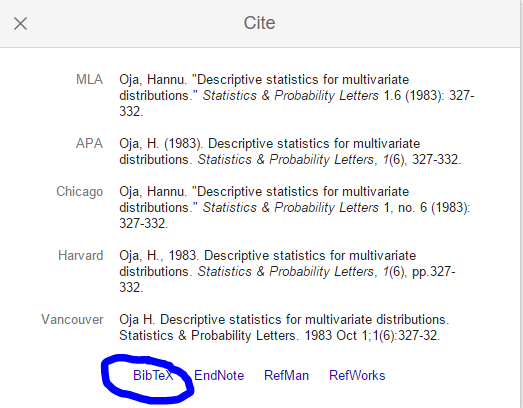
\includegraphics[width=1\textwidth]{figures/hasiltandakutip}}
        \caption{Pilih Menu Bibtex}
		\label{hasiltandakutip}
\end{figure}

\begin{figure}[ht]
        \centerline{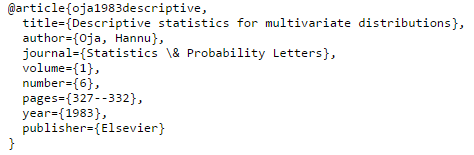
\includegraphics[width=1\textwidth]{figures/hasilbibtex}}
        \caption{Hasil Bibtex}
		\label{hasilbibtex}
\end{figure}
